\documentclass[smaller,dvipsnames,ratio=169,10pt]{beamer}

\usetheme[numbering=fraction,%
          block=fill,%
          sectionpage=progressbar,%
          subsectionpage=progressbar,%
  ]{metropolis} % Use metropolis theme
\setbeamercovered{invisible}

\usepackage[utf8]{inputenc}
\usepackage{xcolor}
\usepackage{xspace}
\usepackage{booktabs}
\usepackage{amssymb}
\usepackage{listings}
\usepackage{todonotes}
\usepackage{csquotes}

\usepackage{tikz,comment}
\usetikzlibrary{shapes.multipart,shapes.geometric,positioning,backgrounds,fit,calc,arrows.meta}

\newcommand{\htw}{\emph{Hunt the Wumpus}\xspace}

\title{Hakuna Matata: A Logic-Based Agent for the \htw Game}
\subtitle{Team White}
\author{Filippo~De~Bortoli \and Aneta~Koleva \and Lorenz~Leutgeb}
\institute{Free University of Bozen-Bolzano\\[2mm] \texttt{\{\href{mailto:filippo.debortoli@stud-inf.unibz.it}{filippo.debortoli},\href{mailto:aneta.koleva@stud-inf.unibz.it}{aneta.koleva},\href{mailto:lorenz.leutgeb@stud-inf.unibz.it}{lorenz.leutgeb}\}\newline @stud-inf.unibz.it}}
\date{2018-06-01}

\begin{document}

  \maketitle

  \begin{frame}{Outline}
    \tableofcontents
  \end{frame}

  \begin{frame}{Task}
    \begin{enumerate}
      \item Develop a logic-based intelligent \alert{agent} that plays the game {\htw}.
      \item The game poses challenges of reasoning with \alert{incomplete information}.
      \item By the nature of the game, the agent must \alert{draw inferences} about the world.
      \item The implemented strategy should \alert{maximize} the achieved \alert{score}.
    \end{enumerate}
  \end{frame}
  
% Explicit explanation of the game is not needed, since the audience is limited and very
% aware of the rules of the game.

  \section{Approach}
	 \begin{frame}{Knowledge About the World}
	  \begin{itemize}
		\item Static, partly-observable.
		\item Initially incomplete, and in many cases always incomplete!
		\item Safety first!
		\item Size of the grid also must be inferred by bumping. 
		\item Safety of rooms is governed by a handful rules.
	  \end{itemize}
	 \end{frame}

 \begin{frame}{Answer Set Programming}
	\begin{itemize}
		\item Previous experience!
		\item Allows to model non-monotonic reasoning through CWA. 
		\item Combines a high-level logic with grounding and solving.
		\item Suitable for processing of incomplete knowledge. 
		\item At each time step, formalize perceptions and knowledge, model of a logic program should yield the next action.
	\end{itemize}
 \end{frame}

  \begin{frame}{World Exploration}  
	 \begin{itemize}
	 	\item Two rooms $a, b$ are \alert{adjacent} if $b$ can be entered from a by \emph{goforward}.
	 	\item \alert{Reachable} are those rooms that are (a) explored, \alert{or} (b) adjacent to an explored room.
	 	\item Unsafety of rooms is inferred from perceptions, and any room that is not unsafe is \alert{safe}.
	 	\item Candidates for exploration are (a) reachable, \alert{and} (b) safe.
	 \end{itemize}
	 
	 But, \ldots\ which candidate is the best, i.e.\ the \alert{goal}?
  \end{frame}
  
  \begin{frame}[allowframebreaks]{A\textsuperscript{$\star$} Search}
	\small{Optimistically estimate number of actions \enquote{between} two rooms:}
	$$\mathsf{cost}\big((s, o), t\big) := \mathsf{taxicab}(s,t) + \mathsf{turns}\big((s, o), t\big)$$ 	    %where $(x, y, o) \in [1;n]^2 \times \{ u, d, l, r\}$ and $t \in [1;n]^2$.
    \begin{center}\vspace{-5mm}\resizebox{0.7\textheight}{0.7\textheight}{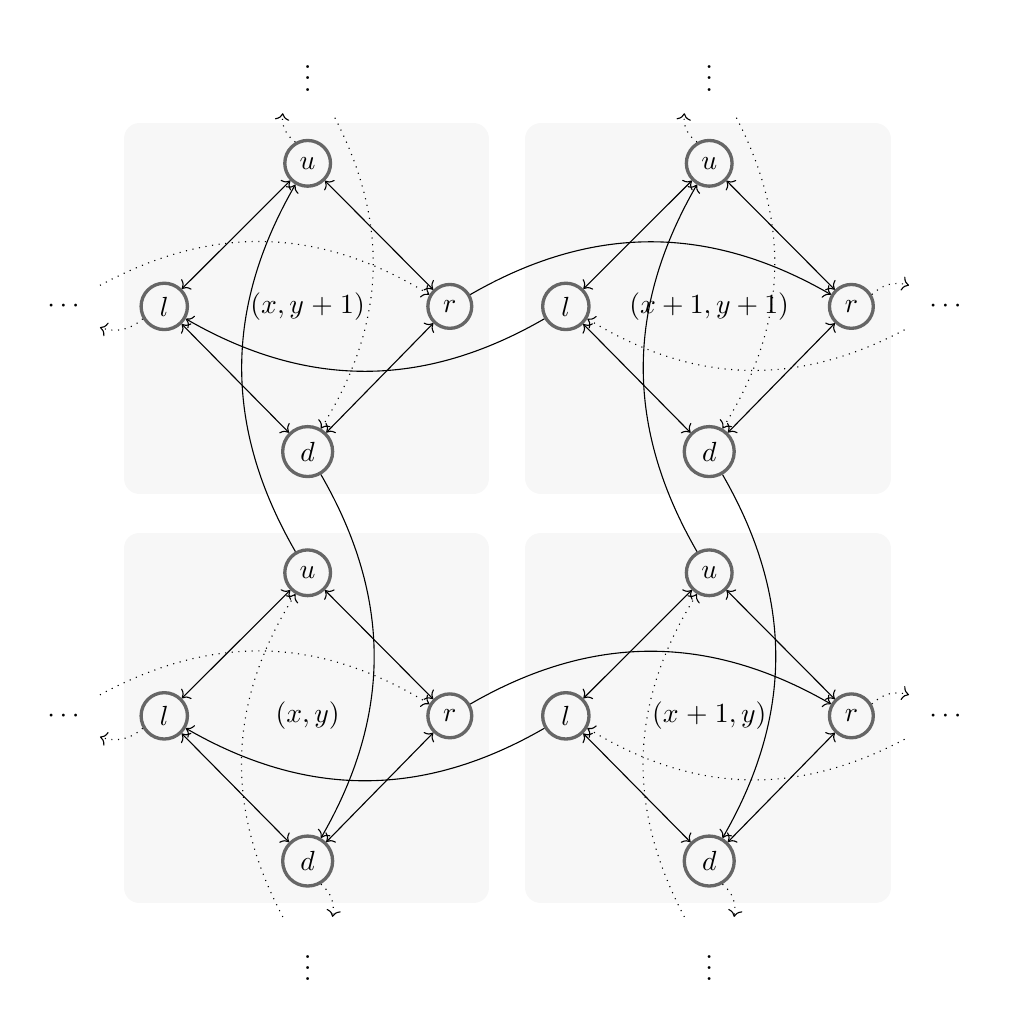
\begin{tikzpicture}[roundnode/.style={circle, draw=black!60, very thick,minimum size=4mm}]
	\begin{scope}
		\node[regular polygon, regular polygon sides=4, align=center, text width={width("$(x + 1, y + 1)$")}] (n11) {$(x, y)$};
		\node[roundnode] (u11) [above=-1mm of n11] {$u$};
		\node[roundnode] (l11) [left=-1mm of n11] {$l$};
		\node[roundnode] (r11) [right=-1mm of n11] {$r$};
		\node[roundnode] (d11) [below=-1mm of n11] {$d$};
		\draw [<->] (u11) -> (l11);
		\draw [<->] (u11) -> (r11);
		\draw [<->] (d11) -> (l11);
		\draw [<->] (d11) -> (r11);
	\end{scope}
		
	\begin{scope}[xshift=5.1cm]
		\node[regular polygon, regular polygon sides=4, align=center, text width={width("$(x + 1, y + 1)$")}] (n21) {$(x + 1, y)$};
		\node[roundnode] (u21) [above=-1mm of n21] {$u$};
		\node[roundnode] (l21) [left=-1mm of n21] {$l$};
		\node[roundnode] (r21) [right=-1mm of n21] {$r$};
		\node[roundnode] (d21) [below=-1mm of n21] {$d$};
		\draw [<->] (u21) -> (l21);
		\draw [<->] (u21) -> (r21);
		\draw [<->] (d21) -> (l21);
		\draw [<->] (d21) -> (r21);
	\end{scope}
		
	\begin{scope}[yshift=5.2cm]
		\node[regular polygon, regular polygon sides=4, align=center, text width={width("$(x + 1, y + 1)$")}] (n12) {$(x, y + 1)$};
		\node[roundnode] (u12) [above=-1mm of n12] {$u$};
		\node[roundnode] (l12) [left=-1mm of n12] {$l$};
		\node[roundnode] (r12) [right=-1mm of n12] {$r$};
		\node[roundnode] (d12) [below=-1mm of n12] {$d$};
		\draw [<->] (u12) -> (l12);
		\draw [<->] (u12) -> (r12);
		\draw [<->] (d12) -> (l12);
		\draw [<->] (d12) -> (r12);
	\end{scope}
		
	\begin{scope}[yshift=5.2cm,xshift=5.1cm]
		\node[regular polygon, regular polygon sides=4, align=center] (n22) {$(x + 1, y + 1)$};
		\node[roundnode] (u22) [above=-1mm of n22] {$u$};
		\node[roundnode] (l22) [left=-1mm of n22] {$l$};
		\node[roundnode] (r22) [right=-1mm of n22] {$r$};
		\node[roundnode] (d22) [below=-1mm of n22] {$d$};
		\draw [<->] (u22) -> (l22);
		\draw [<->] (u22) -> (r22);
		\draw [<->] (d22) -> (l22);
		\draw [<->] (d22) -> (r22);
	\end{scope}
		
	\begin{scope}[xshift=8.1cm]
		\node[regular polygon, regular polygon sides=4] (n31) {$\cdots$};
	\end{scope}
		
	\begin{scope}[yshift=5.2cm,xshift=8.1cm]
		\node[regular polygon, regular polygon sides=4] (n32) {$\cdots$};
	\end{scope}

	\begin{scope}[yshift=8.2cm]
		\node[regular polygon, regular polygon sides=4] (n13) {$\vdots$};
	\end{scope}

	\begin{scope}[yshift=8.2cm,xshift=5.1cm]
		\node[regular polygon, regular polygon sides=4] (n23) {$\vdots$};
	\end{scope}

	\begin{scope}[xshift=-3.1cm]
		\node[regular polygon, regular polygon sides=4] (n01) {$\cdots$};
	\end{scope}

	\begin{scope}[yshift=-3.1cm,xshift=5.1cm]
		\node[regular polygon, regular polygon sides=4] (n20) {$\vdots$};
	\end{scope}

	\begin{scope}[yshift=-3.1cm]
		\node[regular polygon, regular polygon sides=4] (n10) {$\vdots$};
	\end{scope}

	\begin{scope}[yshift=5.2cm,xshift=-3.1cm]
		\node[regular polygon, regular polygon sides=4] (n02) {$\cdots$};
	\end{scope}

	\path [->] (r11) edge [bend left] (r21);
	\path [->] (l21) edge [bend left] (l11);
	\path [->] (u11) edge [bend left] (u12);
	\path [->] (d12) edge [bend left] (d11);
	\path [->] (u21) edge [bend left] (u22);
	\path [->] (d22) edge [bend left] (d21);
	\path [->] (r12) edge [bend left] (r22);
	\path [->] (l22) edge [bend left] (l12);

	\path [->, dotted] (r21) edge [bend left] (n31);
	\path [->, dotted] (r22) edge [bend left] (n32);
	\path [->, dotted] (u12) edge [bend left] (n13);
	\path [->, dotted] (u22) edge [bend left] (n23);
	\path [->, dotted] (l11) edge [bend left] (n01);
	\path [->, dotted] (d11) edge [bend left] (n10);
	\path [->, dotted] (l12) edge [bend left] (n02);
	\path [->, dotted] (d21) edge [bend left] (n20);

	\path [<-, dotted] (l21) edge [bend right] (n31);
	\path [<-, dotted] (l22) edge [bend right] (n32);
	\path [<-, dotted] (d12) edge [bend right] (n13);
	\path [<-, dotted] (d22) edge [bend right] (n23);
	\path [<-, dotted] (r11) edge [bend right] (n01);
	\path [<-, dotted] (u11) edge [bend right] (n10);
	\path [<-, dotted] (r12) edge [bend right] (n02);
	\path [<-, dotted] (u21) edge [bend right] (n20);

	\begin{pgfonlayer}{background}
		\filldraw[line width=4mm,join=round,black!3]
			(u11.north -| r11.east) rectangle (d11.south -| l11.west)
			(u21.north -| r21.east) rectangle (d21.south -| l21.west)
			(u12.north -| r12.east) rectangle (d12.south -| l12.west)
			(u22.north -| r22.east) rectangle (d22.south -| l22.west)
		;
	\end{pgfonlayer}
\end{tikzpicture}
}\vspace{-10mm}\end{center}
	\framebreak
	Given $$\mathsf{cost}\big((s, o), t\big) := \mathsf{taxicab}(s,t) + \mathsf{turns}\big((s, o), t\big)$$\vspace{-5mm}\begin{enumerate}
	    \item Let 0 denote the current location and orientation of the agent.
		\item Choose a \alert{goal} room $g$ s.t.\ $\mathsf{cost}(0, g)$ is minimal.
	    \item Choose the \alert{next} room $n$ s.t.\ $f(n)$ is minimal (A\textsuperscript{$\star$} search): 
	    $$f(n) = f_1(n) + f_2(n)$$ \vspace{-2mm} where
	    \begin{itemize}
	    	\item $f_1(n) := \mathsf{cost}(0, n)$
	    	\item $f_2(n) := \mathsf{cost}((n, o_n), g)$
	    	\item $o_n$ is the orientation the agent would have moving from 0 to $n$.
	    \end{itemize}
	    \item Select an action that will move the agent from 0 closer to $n$.
	\end{enumerate}
  \end{frame}

  \begin{frame}[allowframebreaks]{Modes}
  \begin{center}
  {\large
   OK, exploration is solved, but how to orchestrate all other actions?\\[2cm]
   Introduce \emph{modes} to have better control over the high-level phases of the game!}
   \end{center}
   \framebreak
   \begin{description}
   	\item[Explore]{as long as there are rooms to \alert{explore} and the gold as not been \alert{grabbed}.}
   	\item[Grab]{when \alert{glitter} is perceived.}
   	\item[Kill]{if there are no rooms to \alert{explore}, the gold has not been \alert{grabbed}, and the \alert{arrow} is available, consider: Is the location of the \alert{wumpus} known?
		   	\begin{itemize}
		   		\item Yes. Kill it.
		   		\item No. Attempt to kill it if its location can be inferred from the shot.
		   	\end{itemize}
		   	$\rightarrow$ Let \alert{goal} $:=$ room to shoot from.
    }
   	\item[Escape]{if no other mode is applicable.\newline $\rightarrow$ Let \alert{goal} $:=$ initial room.}
   \end{description}
  \end{frame}

\iffalse
  \begin{frame}{ASP Encoding}
    \begin{center}
      \begin{tabular}{ll}
        \textbf{Predicate} & \textbf{Meaning} \\
        now/3 & position and orientation of the agent \\
        stench/2 & stench has been found in here \\
        wumpusDead/0 & a scream has been perceived \\
        grabbed/0 & glitter perceived, gold has been grabbed \\
      \end{tabular}
    \end{center}
  \end{frame}

  \begin{frame}{Heuristics}
    % TODO.
  \end{frame}
\fi
  \section{Implementation}

  \begin{frame}{Tools of the Trade}
  \emph{Wumpus World Simulator}\footnote{\url{http://www.eecs.wsu.edu/~holder/courses/AI/wumpus/}} translated to Python (C++ optional).

  \begin{center}
  \begin{tabular}{llll}
    \textbf{Tool} & \textbf{Version} & \textbf{Category} & \textbf{Component} \\
    Python & 3.6 & Runtime & Host, Simulator \\
    DLV & 2012-12 & ASP System & Agent\\
  \end{tabular}
  \end{center}
  \end{frame}  
  
	%something more here maybe? it's a section with one slide (diagram)
  \begin{frame}{Architecture of the Implementation}
		\resizebox{1.0\textwidth}{0.55\textheight}{
			
		
			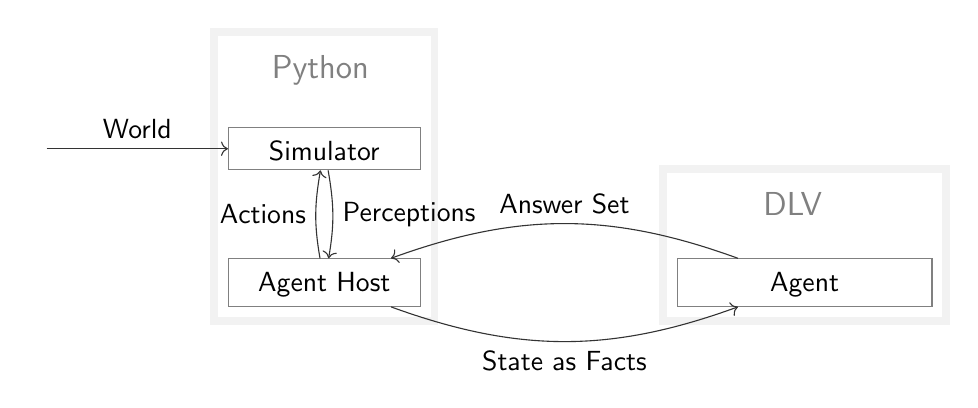
\begin{tikzpicture}[
			node distance=1cm and 5mm,
			every node/.style={font=\sffamily},
			title/.style={font=\color{black!50}\sffamily},
			typetag/.style={rectangle, draw=black!50, font=\sffamily, anchor=west, text height=3mm, align=center}
			]
			
			\node (lp) at (0, -1cm) {};
			\node (as) at (0, -3.2cm) {};
			
			\node (gl) at (3.6cm, 0) [align=center, text width=2.1cm, title] { \large Python };
			
			\node (par) [below=of gl.west, text width=22mm, typetag] { Simulator };
			\node (gro) [below=1.7cm of par.west, text width=22mm, typetag] { Agent Host };
			
			\node (g) [draw=gray!10, line width=1mm, inner sep=5pt, fit={(gl) (par) (gro)}] {};
			
			\node (sl) at (9.6cm, -1.7cm) [align=center, text width=2.7cm, title] { \large DLV };
			
			\node (ngs) [below=of sl.west, text width=3cm, typetag] { Agent };
			
			\node (s) [draw=gray!10, line width=1mm, inner sep=5pt, fit={(sl) (ngs)}] {};
			
			\draw [->, draw=black!80] (gro) to [out=340, in=200] node [midway, below] {State as Facts} (ngs);
			\draw [->, draw=black!80] (ngs) to [out=160, in=20] node [midway, above] {Answer Set} (gro);
			
			\draw [->, draw=black!80] (par) to [out=280, in=80] node [midway, right] {Perceptions} (gro);
			\draw [<-, draw=black!80] (par) to [out=260, in=100] node [midway, left] {Actions} (gro);
			
			\draw [->, draw=black!80] (lp) -- (par) node [midway, above] {World};
			\end{tikzpicture}
	
		}
  \end{frame}

  \begin{frame}{Autopilot}
  	\begin{itemize}
  		\item Reasoning takes the most time.
  		\item Goal room remains stable until it is reached.
  		\item Allow agent to signal activation of autopilot.
  		\item Method: \begin{enumerate}
  		\item Pass safety of rooms to the host.
  		\item Construct graph that reflects the cost function.
  		\item Run BFS to plan a path.
  		\item Execute that path and \enquote{wake up} the agent once arrived.
  		\end{enumerate}
  		\item Prevent planning of paths that pass through unsafe rooms.		  		
		\item Decreases the overall run-time of the agent!
  	\end{itemize}
  \end{frame}
  
  \section{Demonstration}
  
	\begin{frame}[standout]
	\end{frame}

  \section{Evaluation}
  
  \begin{frame}[allowframebreaks]{Perfect Agent}
    \begin{itemize}
      \item Has complete knowledge of the world.
      \item Let $s$ be the initial location and $w$, $t$ the location of wumpus and gold, and $P$ be the set of locations of the pits.
      \item Let $A = \{ turnleft, turnright, goforward, shoot \}$.
      \item Build action graph $G = (V, E, c : E \rightarrow \mathbb{N}_{\infty}, l : E \rightarrow A^+)$:
      \begin{itemize}
      	\item $V := \big\{ (x, y, o) \mid 1 \leq x, y \leq n, \: o \in \{ u, d, l, r\} \big\}$
      	\item $E$ according to horizontal/vertical reachability (as before).
      	\item $c{\big(}(x, y, o), (x', y', o'){\big)} := \begin{cases} \infty & (x', y') \in P \\ 10 & (x,y) = w \text{ and } (x,y) \neq (x',y') \\ 1 & \text{otherwise} \end{cases}$
      	\item For each $e \in E$ introduce a label $l(e)$ as a sequence of actions.
      \end{itemize}

	  \framebreak      
      
      \item Search for shortest path of cost less than 500 from $s$ to $t$.
      \item Does such a path exist? \begin{description}
      	\item[Yes]{Reconstruct and apply actions from $l$, pick up the gold, apply the actions in reverse (minus shooting the arrow), climb.}
      	\item[No]{Climb immediately.}
      \end{description}
      \item Much easier to implement and faster to compute!
      \item Score of this agent as reference for a world.
    \end{itemize}
  \end{frame}


  \begin{frame}[allowframebreaks]{Evaluation}
  	Logic-based agent vs.\ perfect agent scores:
  	\begin{center}
      	\begin{tabular}{rrrrr}
      		\toprule
      		\multicolumn{1}{c}{$n$} & \multicolumn{1}{c}{$N_n$} & \multicolumn{1}{c}{$\bar{\Delta}$} & \multicolumn{1}{c}{$\sigma(\Delta)$} & \multicolumn{1}{c}{$\bar{t} \: [s]$}\\
      		\midrule
      		4 & 160	& 419 & 488 & 0.1440 \\
      		5 & 80  & 464 & 493 & 0.2656 \\
      		6 & 80  & 634 & 474 & 0.4600 \\
      		7 & 40  & 630 & 468 & 2.8005 \\
      		8 & 40  & 653 & 471 & 3.8736 \\
      		9 & 20  & 557 & 490 & 4.7723 \\
      		10 & 20 & 714 & 452 & 11.3828 \\
      		11 & 10 & 785 & 414 & 0.1573 \\
      		12 & 10 & 595 & 498 & 0.5594 \\
      		13 & 5  & 383 & 524 & 0.0158 \\
      		14 & 5  & 600 & 506 & 11.8238 \\
      		\bottomrule\\
      	\end{tabular}
	\end{center}      
      
      \framebreak
      
      Reasons for $\Delta$: 
      \begin{itemize}
        \item Incomplete information!
        \item Possible pits blocking all paths to the gold.
        \item Explores all safely reachable rooms before inferring that the gold is unreachable.
      \end{itemize}
	\end{frame}

  \section{Conclusion}

  \begin{frame}{Conclusion}
  	\begin{itemize}
  		\item Developed an intelligent, logic-based agent that plays the \htw game. 
  		\item Developed an additional agent for evaluation of performance.
  		\item  Additionally, an autopilot component improves the overall run-time of the agent. 
  		\item Successfully carried out a	n empirical evaluation. 
  	\end{itemize}
    
  \end{frame}

  \begin{frame}{Further Extensions}
  
  	\begin{itemize}
	  	 \item Use probability when calculating the next move.
		 \item Variants of \htw
  	  \begin{description}
  		\item[Multiagent]{What if the Wumpus was able to move, or bats where moving in the world?}
	  	\item[Topology]{What if the space was shaped in a different way?}
	  	\item[Continuum]{What if the space was \emph{continuous} and not discrete?}
	  	\item[Oracle]{What if the agent was given the possibility to know the content of a single room without exploring it?}
  	  \end{description}
  	\end{itemize}
  \end{frame}

  \begin{frame}[standout]
    Thank you! Questions?
  \end{frame}

\end{document}
